\documentclass[10pt,a4paper]{article}
\usepackage[a4paper,top=18mm,bottom=19mm,left=19mm,right=19mm,headsep=6mm,footskip=8mm]{geometry}
\usepackage[T1]{fontenc}
\usepackage{libertinus}
\usepackage[final]{microtype}
\usepackage{amsmath,amssymb,mathtools,bm}
\usepackage{booktabs,tabularx,array,longtable,enumitem,multicol,graphicx}
\usepackage[font=small,labelfont=bf]{caption}
\usepackage{tikz}
\usetikzlibrary{arrows.meta,calc,positioning,decorations.pathreplacing,fit,shapes.geometric}
\usepackage{xcolor}
\usepackage[most]{tcolorbox}
\usepackage{fancyhdr,hyperref,titlesec}
\hypersetup{colorlinks=true,linkcolor=blue!40!black,urlcolor=blue!40!black,pdfauthor={PHYS7045 Exam Study Reference},pdftitle={PHYS7045 Past Examination Fully Worked Solutions 2023--2025}}
\definecolor{ink}{HTML}{243449}
\definecolor{muted}{HTML}{536274}
\definecolor{accent}{HTML}{165A75}
\definecolor{soft}{HTML}{F0F5F7}
\definecolor{warm}{HTML}{F7F4ED}
\setlength{\parindent}{0pt}
\setlength{\parskip}{4pt plus 1pt minus 1pt}
\setlength{\emergencystretch}{4em}
\setlist[itemize]{leftmargin=*,topsep=3pt,itemsep=1.5pt,parsep=0pt}
\setlist[enumerate]{leftmargin=*,topsep=3pt,itemsep=2pt,parsep=0pt}
\setcounter{tocdepth}{2}
\setcounter{secnumdepth}{2}
\AtBeginDocument{\color{ink}}
\titleformat{\section}{\Large\bfseries\color{accent}}{\thesection}{.65em}{}
\titleformat{\subsection}{\normalsize\bfseries\color{accent}}{\thesubsection}{.65em}{}
\titleformat{\subsubsection}{\normalsize\bfseries\color{ink}}{\thesubsubsection}{.65em}{}
\titlespacing*{\section}{0pt}{13pt plus 3pt minus 2pt}{5pt}
\titlespacing*{\subsection}{0pt}{10pt plus 3pt minus 1pt}{4pt}
\titlespacing*{\subsubsection}{0pt}{7pt plus 2pt minus 1pt}{3pt}
\pagestyle{fancy}
\fancyhf{}
\fancyhead[L]{\small\color{muted}PHYS7045 \textbar\ Past Exams 2023--2025}
\fancyhead[R]{\small\color{muted}Fully Worked Solutions}
\fancyfoot[C]{\small\color{muted}\thepage}
\renewcommand{\headrulewidth}{0.25pt}
\newtcolorbox{idea}{colback=soft,colframe=accent!35!white,boxrule=.4pt,arc=1.5mm,left=2mm,right=2mm,top=1mm,bottom=1mm,before skip=5pt,after skip=5pt,breakable}
\newtcolorbox{examtip}{colback=warm,colframe=black!16,boxrule=.4pt,arc=1.5mm,left=2mm,right=2mm,top=1mm,bottom=1mm,before skip=5pt,after skip=5pt,breakable}
\newcommand{\ket}[1]{\left\lvert #1\right\rangle}
\newcommand{\bra}[1]{\left\langle #1\right\rvert}
\newcommand{\braket}[2]{\left\langle #1\middle\vert #2\right\rangle}
\newcommand{\Tr}{\operatorname{Tr}}
\newcommand{\I}{\mathbb{I}}
\newcommand{\ee}{\mathrm{e}}
\newcommand{\dd}{\mathrm{d}}
\newcommand{\D}{\mathcal{D}}
\newcommand{\wt}{\operatorname{wt}}
\newcommand{\synd}{\operatorname{synd}}
\newcommand{\X}{\sigma_x}
\newcommand{\Y}{\sigma_y}
\newcommand{\Z}{\sigma_z}
\newcommand{\red}[1]{\textcolor{accent}{#1}}
\begin{document}
\begin{center}
{\huge\bfseries PHYS7045: Quantum Technologies}\par\vspace{2mm}
{\Large\color{accent}Past Examination Papers --- Full Worked Solutions}\par\vspace{2mm}
{\small 2023 \quad\textbullet\quad 2024 \quad\textbullet\quad 2025}\par\vspace{2mm}
{\small Core Part A and advanced Part B, with assumptions, physical explanation and checks}
\end{center}
\begin{idea}
\textbf{How to use these solutions.} Start each question with the original paper, attempt the problem, then compare your method to the explanation here. We retain each year's question numbering and explicitly distinguish \emph{error detection from correction}, \emph{global from relative phases}, and \emph{idealised gate models from physical pulse details}. Our state and operator conventions are stated locally rather than silently changed.
\end{idea}
\tableofcontents
\begin{examtip}
\textbf{Important source note.} The worked problems are referenced to the original exam PDFs in \texttt{source\_material/past\_exams/2023--2025/}. The 2024 Rydberg problem does not give laser detunings or pulse envelopes; the idealised effective-pulse answer is presented with that limitation made explicit. These are independently derived study solutions, not an official examiner marking key.
\end{examtip}
% All questions from Semester Two 2023, including Part B.
\clearpage
\section{2023 examination}
\subsection{Question 1 --- M\o lmer--S\o rensen trapped-ion gate}
\begin{idea}
\textbf{Physics.} Two ions couple to the same quantised vibrational mode. A bichromatic laser drives red and blue sidebands with opposite detunings $\pm\delta$, creating an effective two-photon transition $\ket{gg,n}\leftrightarrow\ket{ee,n}$ without permanently populating the intermediate phonon states. The cancellation of factors $n$ and $n+1$ is the key to the gate's relative insensitivity to thermal motion.
\end{idea}
\subsubsection*{Part A1. Single-ion red and blue sidebands}
With electronic states $\ket g,\ket e$, harmonic-motion state $\ket n$, Lamb--Dicke factor $\eta$, and bare carrier Rabi frequency $\Omega$, the first-order sideband Hamiltonians are, up to laser phases,
\begin{align}
H_{\rm red}&=\frac{\hbar\eta\Omega_r}{2}(\sigma_+a+\sigma_-a^\dagger),&
H_{\rm blue}&=\frac{\hbar\eta\Omega_b}{2}(\sigma_+a^\dagger+\sigma_-a).
\end{align}
The ladder operators satisfy $a\ket n=\sqrt n\ket{n-1}$ and $a^\dagger\ket n=\sqrt{n+1}\ket{n+1}$. Therefore
\begin{align}
\text{red: }&\ket{g,n}\longleftrightarrow\ket{e,n-1},& \Omega_{r,n}&=\eta\Omega_r\sqrt n,\label{eq:23red}\\
\text{blue: }&\ket{g,n}\longleftrightarrow\ket{e,n+1},&\Omega_{b,n}&=\eta\Omega_b\sqrt{n+1}.\label{eq:23blue}
\end{align}
A red-sideband pulse cannot excite $\ket{g,0}$ (there is no phonon to remove). For equal laser strengths $\Omega_r=\Omega_b=\Omega_0$, these become $\eta\Omega_0\sqrt n$ and $\eta\Omega_0\sqrt{n+1}$ respectively.

\subsubsection*{Part A2. Two alternative two-photon pathways}
The figure in the paper contains two families of virtual intermediate states. One creates a phonon first (the $n+1$ path), and the other removes one first (the $n-1$ path):
\begin{figure}[htbp]
\centering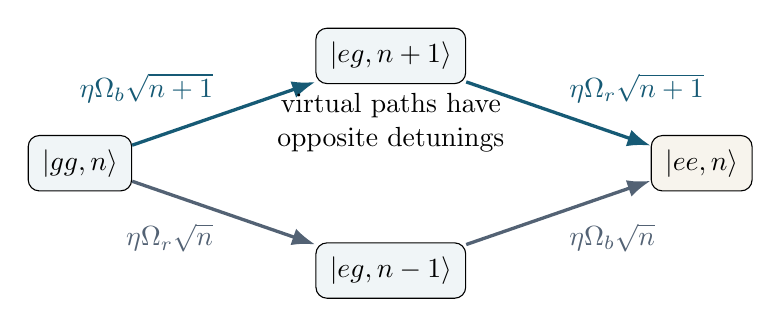
\begin{tikzpicture}[>=Latex,scale=0.94]
 \node[draw,rounded corners,fill=soft,inner sep=5pt] (a) at (0,0) {$\ket{gg,n}$};
 \node[draw,rounded corners,fill=soft,inner sep=5pt] (b) at (4.2,1.45) {$\ket{eg,n+1}$};
 \node[draw,rounded corners,fill=soft,inner sep=5pt] (c) at (4.2,-1.45) {$\ket{eg,n-1}$};
 \node[draw,rounded corners,fill=warm,inner sep=5pt] (d) at (8.4,0) {$\ket{ee,n}$};
 \draw[very thick,accent,->] (a)--(b) node[midway,above left] {$\eta\Omega_b\sqrt{n+1}$};
 \draw[very thick,accent,->] (b)--(d) node[midway,above right] {$\eta\Omega_r\sqrt{n+1}$};
 \draw[very thick,muted,->] (a)--(c) node[midway,below left] {$\eta\Omega_r\sqrt n$};
 \draw[very thick,muted,->] (c)--(d) node[midway,below right] {$\eta\Omega_b\sqrt n$};
 \node[align=center] at (4.2,0.55) {virtual paths have\\ opposite detunings};
\end{tikzpicture}
\caption{The two interfering second-order paths between $\ket{gg,n}$ and $\ket{ee,n}$. Either ion could be excited first; the same $n$-dependence appears for both orderings.}
\end{figure}
The question supplies the second-order two-photon Rabi rule $\Omega_{2\gamma}=\Omega_1\Omega_2/(2\delta_{\rm path})$. If the upper ($n+1$) intermediate state has detuning $+\delta$ and the lower ($n-1$) state $-\delta$, their \emph{signed} contributions are
\begin{equation}\label{eq:23MSpaths}
\Omega_{\rm upper}=2\times\frac{\eta^2\Omega_r\Omega_b(n+1)}{2\delta}=\frac{\eta^2\Omega_r\Omega_b(n+1)}{\delta},\qquad
\Omega_{\rm lower}=-2\times\frac{\eta^2\Omega_r\Omega_b n}{2\delta}=-\frac{\eta^2\Omega_r\Omega_b n}{\delta}.
\end{equation}
Choosing the opposite detuning sign convention reverses both signs and has no effect on the magnitude. The diagram also includes the corresponding pathway with ions $A$ and $B$ exchanged; both orderings contribute equally and must be summed.

\subsubsection*{Part A3. Why the result is independent of phonon occupation}
The upper and lower path families (each summed over both ion orderings) add \emph{coherently}, including their detuning signs:
\begin{equation}\boxed{\displaystyle
\Omega_{\rm eff}=\left|\Omega_{\rm upper}+\Omega_{\rm lower}\right|
=\frac{\eta^2|\Omega_r\Omega_b|}{|\delta|}\big|(n+1)-n\big|
=\frac{\eta^2|\Omega_r\Omega_b|}{|\delta|}.}\label{eq:23MS}
\end{equation}
There is no residual $n$ dependence. \emph{Why?} The factor for creating then annihilating a phonon is $(n+1)$, while annihilating then creating has factor $n$. Their oppositely detuned amplitudes cancel the $n$-dependent terms. This requires the regime where the detuned intermediate levels remain virtual ($|\delta|$ larger than the associated sideband couplings) and other approximations remain valid.

\subsubsection*{Part B(a). Pulse for a maximally entangled Bell state}
Within the effective subspace $\{\ket{gg,n},\ket{ee,n}\}$ take
\begin{equation}H_{\rm eff}=\frac{\hbar\Omega_{\rm eff}}2\left(\ee^{i\chi}\ket{ee}\bra{gg}+\ee^{-i\chi}\ket{gg}\bra{ee}\right).\end{equation}
Starting in $\ket{gg,n}$, the evolution is
\begin{equation}
\ket{\psi(t)}=\cos\frac{\Omega_{\rm eff}t}{2}\ket{gg,n}
-i\ee^{i\chi}\sin\frac{\Omega_{\rm eff}t}{2}\ket{ee,n}.
\end{equation}
Equal-magnitude coefficients require $\Omega_{\rm eff}t=\pi/2$ for the first such pulse:
\begin{equation}\boxed{t_{\rm Bell}=\frac{\pi}{2\Omega_{\rm eff}},\qquad
\ket{\psi(t_{\rm Bell})}=\frac{\ket{gg}-i\ee^{i\chi}\ket{ee}}{\sqrt2}\otimes\ket n.}\end{equation}
This is maximally entangled because tracing either ion gives $\I/2$. The relative phase is set by the optical phase and can be corrected locally. \textbf{Note:} the gate is insensitive to the \emph{initial} $n$ at this effective order; this does not mean it is unaffected by heating or laser noise.

\subsection{Question 2 --- A six-qubit stabiliser code}
The source table, transcribed from page 3 of the 2023 paper, is
\begin{center}\small
\begin{tabular}{@{}c*{6}{c}@{}}\toprule
&1&2&3&4&5&6\\\midrule
$S_1$&Z&I&Z&I&I&I\\
$S_2$&X&Z&Y&Y&X&I\\
$S_3$&X&X&X&X&Z&I\\
$S_4$&I&Z&Z&X&I&X\\
$S_5$&X&Y&X&Y&I&Z\\\bottomrule
\end{tabular}\end{center}
There are five independent commuting stabilisers on six qubits, so $k=6-5=1$ logical qubit is encoded.

\subsubsection*{Part A1. Should $S_1$ commute with the others?}
Yes: generators of a valid stabiliser group must commute so that the code has simultaneous $+1$ eigenspaces. The rule is to count positions where two Pauli factors are \emph{different and neither is $I$}. For $S_1=ZIZIII$:
\begin{center}\small
\begin{tabular}{@{}lll@{}}\toprule Pair & Anticommuting qubit positions & Result\\\midrule
$S_1,S_2$ & 1 ($Z/X$), 3 ($Z/Y$) & 2, commute\\
$S_1,S_3$ & 1 ($Z/X$), 3 ($Z/X$) & 2, commute\\
$S_1,S_4$ & none & 0, commute\\
$S_1,S_5$ & 1 ($Z/X$), 3 ($Z/X$) & 2, commute\\\bottomrule
\end{tabular}\end{center}
In each case $S_1S_j=(-1)^{\text{even}}S_jS_1=S_jS_1$. The remaining stabilisers also commute pairwise, so the code is consistent.

\subsubsection*{Part A2. Check the given logical $Z_L=XYYXII$}
Test $Z_L$ against each generator: the local anticommuting positions are
\begin{center}\small
\begin{tabular}{@{}ccccc@{}}\toprule
$S_1$&$S_2$&$S_3$&$S_4$&$S_5$\\\midrule
$1,3$&$2,4$&$2,3$&$2,3$&$3,4$\\\bottomrule
\end{tabular}\end{center}
All have two mismatches, hence $[Z_L,S_j]=0$ for every $j$. It is not a product of the stabilisers, so it acts nontrivially on the encoded qubit. The notation \emph{logical $Z$} is a choice of computational logical basis, not a requirement that the physical string contain only $Z$ operators.

\subsubsection*{Part A3--A4. Single $X$ and single $Y$ errors: full syndromes}
Write a syndrome as five bits $b_1b_2b_3b_4b_5$, where $b_j=1$ means $E$ \emph{anticommutes} with $S_j$ and therefore flips its eigenvalue to $-1$.
\begin{center}\small
\begin{tabular}{@{}cccc@{}}\toprule
Qubit $j$&$\synd(X_j)$&$\synd(Y_j)$&$\synd(Z_j)$\\\midrule
1&10000&11101&01101\\
2&01011&01110&00101\\
3&11010&10111&01101\\
4&01001&00110&01111\\
5&00100&01100&01000\\
6&00001&00011&00010\\\bottomrule
\end{tabular}\end{center}
All six $X_j$ errors have nonzero and mutually different syndromes; likewise the six $Y_j$ errors. Therefore each set is \emph{detectable and individually correctable}. The table is obtained by checking each generator position rather than multiplying $64\times64$ matrices.

\subsubsection*{Part A5. Does it correct arbitrary single-qubit $X,Y,Z$?}
The $Z$ syndromes are also nonzero, but $Z_1$ and $Z_3$ have the same syndrome $01101$. This is \emph{not a failure}: $Z_1Z_3=S_1$ is a stabiliser, so the two errors have the same action on every codeword. They are a \emph{degenerate} correctable pair. There are no other collisions between inequivalent errors in the combined table. Therefore
\begin{equation}\boxed{\text{Every single-qubit Pauli error is correctable, so }d\geq3.}\end{equation}
The formal criterion $PE_a^\dagger E_bP=c_{ab}P$ permits indistinguishable error pairs precisely when their product acts as a scalar on the code space (here, a stabiliser).

\subsubsection*{Part B(a). Find logical $X_L=ABABII$}
Choose $A=X$, $B=Z$, giving
\begin{equation}\boxed{X_L=XZXZII.}\end{equation}
For $S_1,\ldots,S_5$, this string has respectively $2,2,2,2,2$ anticommuting positions, so it commutes with the entire stabiliser set. Against the specified $Z_L=XYYXII$, there are three local anticommutations (qubits 2, 3, 4), so
\begin{equation}\boxed{X_LZ_L=-Z_LX_L.}\end{equation}
The alternative $YZYZII$ also satisfies the requested properties. Logical Pauli representatives are not unique, since multiplying by stabilisers preserves their encoded action.

\subsubsection*{Part B(b). Find a lower-weight logical operator and the distance}
Multiply the given logical $Z_L=XYYXII$ by $S_5=XYXYIZ$; the factors on qubits 1--2 cancel, those on 3--4 become $Z$ (the Pauli phases cancel), leaving
\begin{equation}\boxed{Z_L S_5=(XYYXII)(XYXYIZ)=IIZZIZ,\qquad \wt(Z_LS_5)=3.}\end{equation}
This is a weight-3 logical operator because multiplying by a stabiliser does not change the logical action. Hence $d\leq3$. Combined with $d\geq3$ from Part A5:
\begin{equation}\boxed{[[6,1,3]],\qquad d=3.}\end{equation}
\begin{examtip}\textbf{Exam principle.} Equal syndromes imply either a correctable degeneracy or an uncorrectable ambiguity. Multiply the two errors: if their product is a stabiliser, the syndrome collision is harmless; if it is a nontrivial logical operator, it is not.\end{examtip}

\subsection{Question 3 --- Entanglement from a $Y\otimes Y$ Hamiltonian}
The Hamiltonian is $H=\frac{\hbar g}{2}(Y_1+Y_2)^2$, where $Y_1=Y\otimes I$ and $Y_2=I\otimes Y$.
\subsubsection*{Part A1. Derive the unitary}
Since $Y_1^2=Y_2^2=I\otimes I$ and $[Y_1,Y_2]=0$,
\begin{equation}(Y_1+Y_2)^2=2I\otimes I+2Y\otimes Y,\qquad H=\hbar g(I\otimes I+Y\otimes Y).\end{equation}
The two Hamiltonian terms commute, so
\begin{align}
U(t)&=\exp[-igt(I\otimes I+Y\otimes Y)]\\
&=\ee^{-igt}\left[\cos(gt)I\otimes I-i\sin(gt)Y\otimes Y\right],
\end{align}
because $(Y\otimes Y)^2=I\otimes I$. The exam's expression omits the prefactor $\ee^{-igt}$: it is a \emph{global phase}, so the two expressions are physically equivalent, although the displayed expression is not the exact exponential of the full stated Hamiltonian. Thus
\begin{equation}\boxed{U(t)\sim\cos(gt)I\otimes I-i\sin(gt)Y\otimes Y.}\end{equation}

\subsubsection*{Part A2. Time for a maximally entangled state}
Use $Y\ket0=i\ket1$. Then $(Y\otimes Y)\ket{00}=-\ket{11}$, so
\begin{equation}U(t)\ket{00}\sim\cos(gt)\ket{00}+i\sin(gt)\ket{11}.\end{equation}
The Schmidt coefficients have equal magnitude when $gt=\pi/4$ modulo $\pi/2$. The shortest positive time is
\begin{equation}\boxed{t=\frac{\pi}{4g},\qquad \ket{\psi(t)}\sim\frac{\ket{00}+i\ket{11}}{\sqrt2}.}\end{equation}
The phase $i$ is relative, but maximal entanglement is unchanged: either reduced density matrix is $I/2$.

\subsubsection*{Part B(a). Construct a CNOT from this entangling gate}
Let $U_{YY}=\exp(-i\pi Y\otimes Y/4)$ and $V=R_x(\pi/2)\otimes R_x(\pi/2)$. Conjugation rotates $Y$ into $Z$:
\begin{equation}V(Y\otimes Y)V^\dagger=Z\otimes Z,\qquad VU_{YY}V^\dagger=\ee^{-i\pi Z\otimes Z/4}.\end{equation}
Because $\ee^{-i\pi Z\otimes Z/4}=\ee^{-i\pi/4}\operatorname{diag}(1,i,i,1)$, local phase gates $S^\dagger=\operatorname{diag}(1,-i)$ yield
\begin{equation}\boxed{(S^\dagger\otimes S^\dagger)\,VU_{YY}V^\dagger=\ee^{-i\pi/4}\mathrm{CZ}.}\end{equation}
Finally $\mathrm{CNOT}_{1\rightarrow2}=(I\otimes H)\mathrm{CZ}(I\otimes H)$, with $H=(X+Z)/\sqrt2$. The factor $\ee^{-i\pi/4}$ is global and irrelevant. The construction is \emph{local rotations $\to$ entangling $YY$ pulse $\to$ local phase gates $\to$ CNOT basis change}.
% All questions from Semester Two 2024, including Part B.
\clearpage
\section{2024 examination}
\subsection{Question 1 --- The five-qubit stabiliser code}
The given generators and candidate logical $X_L$ are
\begin{align*}
S_1&=ZZZII, &S_2&=IIZZZ,\\
S_3&=XIXXI, &S_4&=IXXIX, & X_L&=XXIII.
\end{align*}
There are five data qubits and four independent commuting checks, so $k=5-4=1$ encoded qubit.

\subsubsection*{Part A1. Does $S_1$ commute with the other generators?}
Any two stabiliser generators must commute. Here $S_1=ZZZII$ and $S_2=IIZZZ$ overlap at qubit 3 with $Z/Z$, so commute. Against $S_3=XIXXI$, the only anticommutes occur on qubits 1 and 3 ($Z/X$ twice); against $S_4=IXXIX$, they occur on qubits 2 and 3. Every count is even, hence
\begin{equation}[S_1,S_2]=[S_1,S_3]=[S_1,S_4]=0.\end{equation}
For completeness, $S_2$ also has two mismatches with each $X$-type check, and $S_3$ commutes with $S_4$, so all four can be measured as a stabiliser family.

\subsubsection*{Part A2. Verify $X_L=XXIII$}
The candidate $X_L$ has two $Z/X$ mismatches with $S_1$ (qubits 1,2); none with $S_2$, and no mismatches with $S_3,S_4$ because those factors are either $X$ or $I$. Thus
\begin{equation}\boxed{[X_L,S_j]=0\quad(j=1,2,3,4).}\end{equation}
It is not a stabiliser product (its eigenvalues distinguish logical states), so it is a valid nontrivial encoded Pauli.

\subsubsection*{Part A3--A4. Syndromes for all individual $X$, $Z$ and $Y$ errors}
Use $b_j=1$ for an error anticommute with $S_j$ ($-1$ measurement result), with bits ordered $S_1S_2S_3S_4$. Position-by-position anticommutation gives
\begin{center}\small
\begin{tabular}{@{}cccc@{}}\toprule Qubit&$\synd(X_j)$&$\synd(Y_j)$&$\synd(Z_j)$\\\midrule
1&1000&1010&0010\\
2&1000&1001&0001\\
3&1100&1111&0011\\
4&0100&0110&0010\\
5&0100&0101&0001\\\bottomrule
\end{tabular}\end{center}
\textbf{Detection.} Every one of the 15 single-qubit Pauli errors produces a nonzero syndrome. Thus every such error is detectable.

\textbf{Correction of bit flips.} $X_1$ and $X_2$ have the same syndrome $1000$, while $X_4$ and $X_5$ both give $0100$. These cannot be corrected unambiguously: for example, $X_1X_2=X_L$ is a \emph{nontrivial logical operator}, not a stabiliser. Choosing the wrong correction introduces a logical error. Hence single $X$ errors are \emph{detectable but not all correctable}.

\textbf{Correction of phase flips.} $Z_1$ and $Z_4$ both give $0010$, and $Z_2$ and $Z_5$ give $0001$. These collisions are likewise harmful: $Z_1Z_4$ is a nontrivial logical $Z$ (shown below). Single $Z$ errors are also \emph{detectable but not all correctable}.

\subsubsection*{Part A5. Can the code correct an arbitrary single-qubit Pauli error?}
No. It detects all such errors, but the syndrome collisions among inequivalent single-qubit $X$ and $Z$ errors violate the correctability requirement. A full set of single $Y$ errors happens to have distinct syndromes, but that does not rescue correction of the entire $\{X_j,Y_j,Z_j\}$ family.
\begin{equation}\boxed{\text{All single Pauli errors detectable; arbitrary single Pauli errors not all correctable.}}\end{equation}
Since every weight-1 Pauli has a nonzero syndrome, there is no undetectable weight-1 logical operator and $d\ge2$.

\subsubsection*{Part B(a). Construct logical $Z_L$}
Try $Z_L=ZIIZI=Z_1Z_4$. It commutes with $S_1,S_2$, which consist solely of $Z$s. Against $S_3=XIXXI$ it anticommutes locally twice (qubits 1 and 4), so commutes overall. Against $S_4=IXXIX$ there are no mismatches. Therefore $[Z_L,S_j]=0$ for all $j$.
With $X_L=XXIII$, there is exactly one $X/Z$ mismatch, on qubit 1. Thus
\begin{equation}\boxed{Z_L=ZIIZI,\qquad X_LZ_L=-Z_LX_L.}\end{equation}
Equally valid is $Z_L=IZIIZ$, which differs by stabiliser multiplication. The mutually anticommuting representatives reproduce the expected logical Pauli algebra.

\subsubsection*{Part B(b). Calculate the code distance}
Both $X_L=XXIII$ and $Z_L=ZIIZI$ have weight 2, so $d\le2$. Part A5 ruled out undetectable weight-1 Paulis, so $d\ge2$. Hence
\begin{equation}\boxed{[[5,1,2]],\qquad d=2,\qquad t=\left\lfloor\frac{d-1}{2}\right\rfloor=0.}\end{equation}
A distance-2 code detects \emph{any} single-qubit Pauli error but guarantees correction of none for an unrestricted noise model. That is precisely consistent with the ambiguous syndromes found above.
\begin{examtip}\textbf{Key contrast with 2023.} In the 2023 code, the collision $Z_1\sim Z_3$ is harmless because $Z_1Z_3$ is a stabiliser. In this 2024 code, $X_1\sim X_2$ is harmful because $X_1X_2$ is logical $X_L$. The syndrome pattern alone is insufficient until you check the \emph{difference operator}.\end{examtip}

\subsection{Question 2 --- Dual-rail beam splitter and probabilistic teleportation}
\subsubsection*{Part A1. Implement a dual-rail Hadamard}
The logical basis is $\ket{0_L}=\ket{1,0}=a^\dagger\ket{\mathrm{vac}}$, $\ket{1_L}=\ket{0,1}=b^\dagger\ket{\mathrm{vac}}$. The paper gives
\begin{equation}
\begin{split}
a^\dagger&\mapsto a^\dagger\cos\theta+b^\dagger\ee^{i\phi}\sin\theta,\\
b^\dagger&\mapsto b^\dagger\cos\theta-a^\dagger\ee^{-i\phi}\sin\theta.
\end{split}
\end{equation}
Apply these transformations to each logical basis state. In the \emph{output logical basis}, the induced two-dimensional unitary has columns given by the transformed basis vectors:
\begin{equation}\label{eq:24bs}
B(\theta,\phi)=\begin{pmatrix}
\cos\theta&-\ee^{-i\phi}\sin\theta\\
\ee^{i\phi}\sin\theta&\cos\theta
\end{pmatrix}.
\end{equation}
Taking $\theta=\pi/4$ and $\phi=0$ gives
\begin{equation}B(\pi/4,0)=\frac1{\sqrt2}\begin{pmatrix}1&-1\\1&1\end{pmatrix}=HZ,\qquad H=\frac1{\sqrt2}\begin{pmatrix}1&1\\1&-1\end{pmatrix}.\end{equation}
Therefore add a $\pi$ phase shift on the second input rail ($Z=\mathrm{diag}(1,-1)$), so
\begin{equation}\boxed{H=B(\pi/4,0)Z.}\end{equation}
\emph{Subtlety:} No choice of $\theta,\phi$ in the given bare $B$ alone equals the displayed $H$ exactly, because both diagonal entries of $B$ are equal whereas $H$ has opposite diagonal entries. A rail phase shifter (or equivalent port-phase convention) supplies the required sign. Thus the physical Hadamard is a balanced beam splitter \emph{plus a relative rail phase}.
\begin{figure}[htbp]\centering
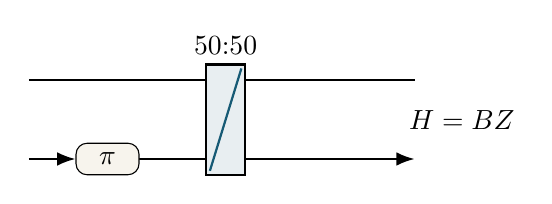
\begin{tikzpicture}[>=Latex]
\draw[thick] (0,1)--(2.4,1) (0,0)--(2.4,0);
\draw[fill=accent!10,thick] (1.05,-.2) rectangle (1.55,1.2);
\draw[thick,accent] (1.1,-.15)--(1.5,1.15);
\node[above] at (1.3,1.2) {50:50};
\node[draw,rounded corners,fill=warm,minimum width=.8cm,minimum height=.4cm] (z) at (-.2,0) {$\pi$};
\draw[->,thick] (-1.2,1)--(0,1) (-1.2,0)--(z.west);
\draw[->,thick] (2.4,1)--(3.7,1) (2.4,0)--(3.7,0);
\node at (4.3,.5) {$H=BZ$};
\end{tikzpicture}
\caption{A balanced beam splitter plus a phase shift on one rail implements an exact logical Hadamard with the stated convention.}
\end{figure}

\subsubsection*{Part B(a). Show the single-rail teleportation succeeds with probability $1/2$}
\textbf{Be careful about the encoding.} The circuit in the paper uses the Fock basis $\{\ket0,\ket1\}$ of an \emph{individual optical mode} for the state to be teleported; that is a \emph{single-rail} input, although Part A concerns dual-rail qubits. Label the input mode $0$, Alice's resource mode $1$, and Bob's output mode $2$.

The input and entangled resource are
\begin{equation}
\ket{\psi}_0=\alpha\ket0_0+\beta\ket1_0,\quad
\ket{t_1}_{12}=\frac{\ket{0,1}_{12}+\ket{1,0}_{12}}{\sqrt2},\quad
|\alpha|^2+|\beta|^2=1.
\end{equation}
Expand \emph{before} the final 50:50 beam splitter:
\begin{align}
\ket\Psi_{012}=\frac1{\sqrt2}(&\alpha\ket{0,0}_{01}\ket1_2+\alpha\ket{0,1}_{01}\ket0_2\\
&+\beta\ket{1,0}_{01}\ket1_2+\beta\ket{1,1}_{01}\ket0_2).
\end{align}
Only the middle two terms have exactly one photon in Alice's measured modes $0$ and $1$. The projector onto $n_0+n_1=1$ gives the unnormalised state
\begin{equation}
\ket{\Psi_{\rm one}}=\frac1{\sqrt2}(\alpha\ket{0,1}_{01}\ket0_2+\beta\ket{1,0}_{01}\ket1_2).
\end{equation}
Its squared norm is $(|\alpha|^2+|\beta|^2)/2=1/2$, already proving the total success probability. To find Bob's conditional state, use the balanced beam-splitter convention
\begin{equation}
\ket{1,0}\mapsto\frac{\ket{1,0}+\ket{0,1}}{\sqrt2},\qquad
\ket{0,1}\mapsto\frac{-\ket{1,0}+\ket{0,1}}{\sqrt2}.
\end{equation}
After Alice's beam splitter, the one-photon sector becomes
\begin{equation}
\frac12\left[\ket{1,0}_{01}(-\alpha\ket0_2+\beta\ket1_2)
+\ket{0,1}_{01}(\alpha\ket0_2+\beta\ket1_2)\right].
\end{equation}
The outcomes in the paper correspond to $n_0=1,n_1=0$ or $n_0=0,n_1=1$. Each occurs with probability $1/4$, independent of $\alpha,\beta$. If $n_0=0,n_1=1$, Bob already has $\ket\psi$. If $n_0=1,n_1=0$, Bob's state is $-\alpha\ket0+\beta\ket1=-Z\ket\psi$, and he applies $Z$ (the extra minus is global).
\begin{center}\small
\begin{tabular}{@{}cccc@{}}\toprule Detector $(n_0,n_1)$&Probability&Bob's state (up to phase)&Correction\\\midrule
$(0,1)$&$1/4$&$\alpha\ket0+\beta\ket1$&$I$\\
$(1,0)$&$1/4$&$\alpha\ket0-\beta\ket1$&$Z$\\
$(0,0)$ or total 2&$1/2$ total&not the desired qubit&failure\\\bottomrule
\end{tabular}\end{center}
\begin{equation}\boxed{P_{\rm success}=P(1,0)+P(0,1)=\frac14+\frac14=\frac12.}\end{equation}
This \emph{heralded} scheme succeeds only when the total photon count at Alice's two detectors is exactly one, as specified. The lower output optical mode carries the teleported state. Passive linear optics here cannot distinguish a complete Bell basis deterministically, which is why failures are unavoidable with this resource/detection setup.

\subsection{Question 3 --- Simultaneous-pulse Rydberg gates}
The original figure shows an $\Omega_1$ drive coupling $\ket0\leftrightarrow\ket r$ on both atoms and an additional $\Omega_2$ drive coupling $\ket1\leftrightarrow\ket r$ \emph{on the target only}. With both colours present, the target can undergo an effective $\ket0\leftrightarrow\ket1$ transition via the Rydberg level, while the control's occupation of $\ket r$ blocks that target transition.

\subsubsection*{Part A1. Pulse areas required}
The desired logic is a \emph{closed control excursion} and a \emph{target bit flip only in the unblocked branch}. Thus:
\begin{itemize}
\item In the branch where control $\ket0$ couples to $\ket r$, the driven control should make a $2\pi$ excursion and return to $\ket0$ (acquiring a phase of $-1$ in the ideal two-level convention).
\item In the branch where the control remains $\ket1$, the target must undergo an effective $\pi$ rotation between its computational states $\ket0,\ket1$, so its population swaps (up to an optical phase).
\item When the control is excited to $\ket r$, blockade shifts the target's intermediate Rydberg state by $\Delta_{rr}$, suppressing its effective flip if $|\Delta_{rr}|\gg\Omega_1,\Omega_2$ (in angular-frequency units).
\end{itemize}
For a simple \emph{effective} two-level description, the conditions are $\int\Omega_{1,c}\,\dd t=2\pi$ for the control excursion and $\int\Omega_{\rm eff,t}\,\dd t=\pi$ for the unblocked target. \textbf{The given figure does not specify pulse envelopes, detunings or coupling ratios, so it does not uniquely determine the numerical $\Omega_1,\Omega_2$ pulse durations.} In a resonant three-level target, an exact swap instead corresponds to a $2\pi$ bright-state cycle; this is explained below.

\subsubsection*{Part A2. Show the four computational-basis cases}
In the ideal blockaded effective model, the gate acts as follows (controls written first):
\begin{center}\small
\begin{tabular}{@{}llll@{}}\toprule
Input&Control response&Target response&Logical output\\\midrule
$\ket{1_c0_t}$&control dark&unblocked flip&$\ket{1_c1_t}$\\
$\ket{1_c1_t}$&control dark&unblocked flip&$\ket{1_c0_t}$\\
$\ket{0_c1_t}$&control excursion to $r$&blocked / unchanged&$\ket{0_c1_t}$\\
$\ket{0_c0_t}$&control excursion to $r$&blocked / unchanged&$\ket{0_c0_t}$\\\bottomrule
\end{tabular}\end{center}
The logical map is therefore a CNOT with \emph{control on $\ket1$} (up to conditional phases). To see how phases arise, a resonant $2\pi$ control cycle contributes $-1$ on the control-$0$ sector. In that simple convention, the ideal operation is
\begin{equation}
U_{\rm ideal}= -\ket0\bra0_c\otimes I_t+\ket1\bra1_c\otimes X_t
=-(Z_c\otimes I_t)\,\mathrm{CNOT}_{c\rightarrow t},
\end{equation}
so a single-qubit $Z$ on the control corrects the unwanted relative sign (global $-1$ is irrelevant).

\textbf{Three-level detail.} With $\Omega_1$ and $\Omega_2$ exactly resonant and simultaneous on the target, its Hamiltonian is
\begin{equation}H_t=\frac\hbar2\left(\Omega_1\ket r\bra0+\Omega_2\ket r\bra1+\mathrm{h.c.}\right).
\end{equation}
It couples only the \emph{bright} state $\ket B\propto\Omega_1\ket0+\Omega_2\ket1$ to $\ket r$; the orthogonal dark state is stationary. For equal real couplings, $\ket B=(\ket0+\ket1)/\sqrt2$, $\ket D=(\ket0-\ket1)/\sqrt2$; a $2\pi$ bright-state cycle sends $\ket B\mapsto-\ket B$ and $\ket D\mapsto\ket D$, which is $-X$ on the target basis. That is the physical origin of the effective target swap. A fully simultaneous implementation must coordinate these bright-state and control cycles (often using pulse shaping, detuning or composite sequences); a single equal-amplitude rectangular pulse is not sufficient to satisfy both exact cycles automatically. The question's truth-table argument assumes these pulse conditions have been engineered.

\subsubsection*{Part A3. Technical advantage}
Simultaneous pulses reduce the need to switch and readdress separate consecutive control/target pulses. Fewer independent timing steps can shorten the gate, reduce exposure to decoherence and decrease errors from pulse calibration or beam steering. They trade this for the need to synchronise phases, detunings and the multi-level dynamics.

\subsubsection*{Part B(a). Extend to a three-qubit Toffoli gate}
Place the \emph{target in the middle}, with controls on either side, such that each control blockades the target but the controls are far enough apart not to blockade each other:
\begin{center}
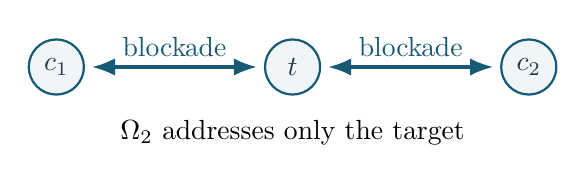
\begin{tikzpicture}[>=Latex]
 \foreach \x/\lab in {0/$c_1$,3/$t$,6/$c_2$}{\draw[fill=soft,draw=accent,thick] (\x,0) circle(.35);\node[text=ink] at (\x,0) {\lab};}
 \draw[very thick,<->,accent] (.45,0)--(2.55,0) node[midway,above] {blockade};
 \draw[very thick,<->,accent] (3.45,0)--(5.55,0) node[midway,above] {blockade};
 \node[below] at (3,-.55) {$\Omega_2$ addresses only the target};
\end{tikzpicture}
\end{center}
A control in $\ket0$ can be driven to $\ket r$, blocking the target. Only when \emph{both} controls are in $\ket1$ does neither become excited, allowing the target's effective flip. After returning the control excitations, the computational action is
\begin{equation}\boxed{\ket{c_1,c_2,t}\longmapsto\ket{c_1,c_2,t\oplus(c_1c_2)}.}\end{equation}
This is Toffoli (CCNOT), up to phases that must be compensated as in Part A. Explicitly, the eight computational inputs map as follows:
\begin{center}\small
\begin{tabular}{@{}c*{8}{c}@{}}\toprule
Input&$000$&$001$&$010$&$011$&$100$&$101$&$110$&$111$\\\midrule
Output&$000$&$001$&$010$&$011$&$100$&$101$&$111$&$110$\\\bottomrule
\end{tabular}\end{center}
The geometry is essential: if the two controls also blockaded each other, the simple argument that they can be independently excited would fail. Exact experimental pulse calibration remains a separate requirement.
% All questions from Semester Two 2025, including Part B.
\clearpage
\section{2025 examination}
\subsection{Question 1 --- The nine-qubit Shor-type stabiliser code}
The given eight stabilisers are
\begin{align*}
S_1&=Z_1Z_2,&S_2&=Z_2Z_3,&S_3&=Z_4Z_5,&S_4&=Z_5Z_6,\\
S_5&=Z_7Z_8,&S_6&=Z_8Z_9,&S_7&=X_1X_2X_3X_4X_5X_6,&S_8&=X_4X_5X_6X_7X_8X_9.
\end{align*}
They define three blocks $\{1,2,3\}$, $\{4,5,6\}$, and $\{7,8,9\}$. There are $n=9$ qubits and $r=8$ independent stabilisers, so $k=1$ logical qubit.

\subsubsection*{Part A1. Should $S_1$ commute with the others?}
Yes, as every pair of stabiliser generators must commute. For $S_1=Z_1Z_2$, the other $Z$ checks $S_2,\ldots,S_6$ obviously commute (they contain only $Z$ or $I$). Against $S_7=X_1X_2X_3X_4X_5X_6$ there are \emph{two} local $Z/X$ anticommutes (qubits 1 and 2), giving $(-1)^2=+1$. Against $S_8$, the supports are disjoint. Thus
\begin{equation}\boxed{[S_1,S_j]=0\quad\text{for }j=2,\ldots,8.}\end{equation}
The same even-overlap rule proves commutation among the complete generating set. For instance, $S_7$ overlaps with $S_3$ on qubits 4 and 5 (two $X/Z$ anticommutes), and $S_7,S_8$ are both products of $X$s and commute.

\subsubsection*{Part A2. Find a logical $X_L$}
Choose one physical $Z$ from each three-qubit block:
\begin{equation}\boxed{X_L=Z_1Z_4Z_7=ZIIZIIZII.}\end{equation}
It commutes with the six $Z$-type generators. Against $S_7$, it anticommutes locally on qubits 1 and 4 (two positions), while against $S_8$ it anticommutes locally on qubits 4 and 7 (two positions). It therefore commutes with all stabilisers. It is \emph{not} itself a stabiliser: it changes the encoded logical state. Why call a product of physical $Z$s a logical $X$? Because the codewords are products of GHZ blocks:
\begin{equation}\ket{0_L}=\frac{(\ket{000}+\ket{111})^{\otimes3}}{2\sqrt2},\quad
\ket{1_L}=\frac{(\ket{000}-\ket{111})^{\otimes3}}{2\sqrt2}.\end{equation}
Applying $Z$ to one physical qubit of each block exchanges $\ket{0_L}\leftrightarrow\ket{1_L}$, which is exactly logical $X$.

\subsubsection*{Part A3. Detect and correct a single bit flip $X_j$}
An $X_j$ anticommutes with the $Z$ checks that contain qubit $j$. Thus the first six syndrome bits locate the specific bit flip within its block. The last two checks, being $X$-type, commute with $X_j$ and yield $+1$.
\begin{center}\small
\begin{tabular}{@{}cccl@{}}\toprule
Error&$S_1\cdots S_6$ ($1=-$)&$S_7S_8$&Interpretation\\\midrule
$X_1$&100000&00&first qubit, block 1\\
$X_2$&110000&00&middle qubit, block 1\\
$X_3$&010000&00&third qubit, block 1\\
$X_4$&001000&00&first qubit, block 2\\
$X_5$&001100&00&middle qubit, block 2\\
$X_6$&000100&00&third qubit, block 2\\
$X_7$&000010&00&first qubit, block 3\\
$X_8$&000011&00&middle qubit, block 3\\
$X_9$&000001&00&third qubit, block 3\\\bottomrule
\end{tabular}\end{center}
All nine syndromes are nonzero and different, so a single $X$ error is \emph{detected and corrected}: measure the eight generators, infer $j$, and apply $X_j$ as the recovery.

\subsubsection*{Part A4. Detect and correct a single phase error $Z_j$}
A $Z_j$ commutes with $S_1,\ldots,S_6$. It anticommutes with $S_7$ and/or $S_8$ according to which three-qubit block contains $j$:
\begin{center}\small
\begin{tabular}{@{}ccc@{}}\toprule
Location of $Z_j$&$S_7S_8$ syndrome&Decoder example\\\midrule
Block 1: $j=1,2,3$&10&apply $Z_1$\\
Block 2: $j=4,5,6$&11&apply $Z_4$\\
Block 3: $j=7,8,9$&01&apply $Z_7$\\\bottomrule
\end{tabular}\end{center}
The syndrome identifies the \emph{block}, not the exact qubit. Nevertheless the error is correctable because $Z_1Z_2=S_1$ and $Z_2Z_3=S_2$, so $Z_1$, $Z_2$ and $Z_3$ differ only by stabilisers on the code space; similarly in the other blocks. This is another example of \emph{degeneracy}: distinct physical errors are equivalent logical errors.

\subsubsection*{Part A5. Arbitrary single $X$, $Y$ or $Z$}
A $Y_j$ is proportional to $X_jZ_j$, so it combines the \emph{position-specific} first-six-bit $X$ syndrome with the \emph{block-specific} two-bit $Z$ syndrome. Example: $Y_5$ returns $001100\,11$ and can be corrected by $Y_5$. All weight-1 Pauli errors therefore have sufficient syndrome information to choose a valid recovery, taking degeneracy into account:
\begin{equation}\boxed{\text{The code corrects any one-qubit }X,Y\text{ or }Z\text{ error.}}\end{equation}
Hence its distance must satisfy $d\ge3$.

\subsubsection*{Part B(a). Logical $Z_L$ and Pauli algebra}
A suitable choice is
\begin{equation}\boxed{Z_L=X_1X_2X_3=XXXIIIIII.}\end{equation}
The $X$s on qubits 1,2,3 commute with all $Z$-type checks: each such check overlaps on either zero or two positions. They also commute with $S_7,S_8$ because those are products of $X$ and $I$. The representative is not a stabiliser, because it acts as $+1$ on $\ket{0_L}$ and $-1$ on $\ket{1_L}$.

With $X_L=Z_1Z_4Z_7$, the two logical operators have exactly one differing nonidentity Pauli at a common qubit (qubit 1), therefore
\begin{equation}\boxed{[Z_L,S_j]=0\ (j=1,\ldots,8),\qquad Z_LX_L=-X_LZ_L.}\end{equation}
These are precisely the logical Pauli relationships expected for an encoded qubit.

\subsubsection*{Part B(b). Find the code distance}
The two nontrivial logical operators just constructed each have weight 3. Thus $d\le3$. On the other hand, Part A5 demonstrated correction of every arbitrary single-qubit error, so $d\ge3$. Therefore
\begin{equation}\boxed{[[9,1,3]],\qquad d=3.}\end{equation}
The nine-qubit code is the familiar Shor-type scheme: three blocks protect bit flips internally while the $X$-type checks compare their collective phases.

\subsection{Question 2 --- Trapped-ion three-pulse entangling gate}
Let $\ket{g}=\ket0$ and $\ket e=\ket1$. The qubits are ions $A,B$, with shared phonon number $n$, initially $n=0$. A red-sideband pulse couples the subspace $\ket{e,n}\leftrightarrow\ket{g,n+1}$. With a suitable fixed laser phase, a resonant $\pi$ pulse sends each participating basis state to $-i$ times its partner, and a resonant $2\pi$ pulse returns it with phase $-1$.

\subsubsection*{Part A1. Pulse 1: red-sideband $\pi$ on ion $A$}
Only an excited $A$ with $n=0$ couples, by $\ket{e_A,0}\to-i\ket{g_A,1}$. A ground-state $A$ with $n=0$ cannot be further lowered; it is dark. Therefore
\begin{align*}
\ket{gg,0}&\to\ket{gg,0},&\ket{ge,0}&\to\ket{ge,0},\\
\ket{eg,0}&\to-i\ket{gg,1},&\ket{ee,0}&\to-i\ket{ge,1}.
\end{align*}
This step conditionally maps $A$'s electronic excitation into one shared motional quantum.

\subsubsection*{Part A2. Pulse 2: red-sideband $2\pi$ on $B$ for $g\leftrightarrow a$}
This laser addresses $\ket{g_B,1}\leftrightarrow\ket{a_B,0}$, but not $\ket{e_B,1}$. A $2\pi$ cycle contributes $-1$ \emph{only} to the component with $B=g$ and a phonon available. Consequently
\begin{align*}
\ket{gg,0}&\to\ket{gg,0},&\ket{ge,0}&\to\ket{ge,0},\\
-i\ket{gg,1}&\to+i\ket{gg,1},&-i\ket{ge,1}&\to-i\ket{ge,1}.
\end{align*}
Notice how a phase is acquired conditionally without permanently populating the auxiliary level $\ket a$.

\subsubsection*{Part A3. Pulse 3: red-sideband $\pi$ on $A$ to restore the motion}
The second $A$ pulse sends $\ket{g_A,1}\to-i\ket{e_A,0}$; the two participating branches become
\begin{align*}
+i\ket{gg,1}&\to (+i)(-i)\ket{eg,0}=+\ket{eg,0},\\
-i\ket{ge,1}&\to (-i)(-i)\ket{ee,0}=-\ket{ee,0}.
\end{align*}
The other two input branches remain unchanged. Every output ends with phonon number $n=0$, which is essential for an operation acting \emph{only} on the computational two-qubit space.

\begin{center}\small
\renewcommand{\arraystretch}{1.25}
\begin{tabular}{@{}lllll@{}}\toprule
Input&After $\pi_A$&After $2\pi_B$&After $\pi_A$&Phase\\\midrule
$\ket{gg,0}$&$\ket{gg,0}$&$\ket{gg,0}$&$\ket{gg,0}$&$+1$\\
$\ket{ge,0}$&$\ket{ge,0}$&$\ket{ge,0}$&$\ket{ge,0}$&$+1$\\
$\ket{eg,0}$&$-i\ket{gg,1}$&$+i\ket{gg,1}$&$\ket{eg,0}$&$+1$\\
$\ket{ee,0}$&$-i\ket{ge,1}$&$-i\ket{ge,1}$&$-\ket{ee,0}$&$-1$\\\bottomrule
\end{tabular}\end{center}

\subsubsection*{Part A4. Matrix and gate identification}
In the specified basis $\{\ket{gg},\ket{ge},\ket{eg},\ket{ee}\}$, the complete sequence implements
\begin{equation}\boxed{U=\begin{pmatrix}1&0&0&0\\0&1&0&0\\0&0&1&0\\0&0&0&-1\end{pmatrix}=\mathrm{CZ}.}\end{equation}
It is entangling because a $-1$ phase appears only when both qubits are excited. For example,
\begin{equation}U\ket{+,+}=\frac{\ket{gg}+\ket{ge}+\ket{eg}-\ket{ee}}2,\end{equation}
which has entangled Schmidt structure. The result is unitary and the motion disentangles at the end.

\subsubsection*{Part A5. Construct a CNOT}
Hadamard-conjugate the \emph{target} ion $B$:
\begin{equation}\boxed{\mathrm{CNOT}_{A\to B}=(I_A\otimes H_B)\,\mathrm{CZ}_{AB}\,(I_A\otimes H_B).}\end{equation}
The first target Hadamard turns a conditional phase into a conditional bit flip, and the second restores the computational-basis description. This is an exact gate identity, not merely a similarity in truth tables.

\subsubsection*{Part B(a). Controlled-controlled operation on $A,B,C$}
The controlled-controlled phase gate (CCZ) leaves every computational basis state unchanged except for the three-excitation state:
\begin{equation}\boxed{\mathrm{CCZ}\ket{abc}=(-1)^{abc}\ket{abc},\quad a,b,c\in\{0,1\}.}\end{equation}
Equivalently $\ket{eee}\mapsto-\ket{eee}$ and the other seven states acquire phase $+1$. A Toffoli (CCNOT) follows by Hadamards on the last qubit:
\begin{equation}\mathrm{CCNOT}_{AB\to C}=(I_A\otimes I_B\otimes H_C)\,\mathrm{CCZ}\,(I_A\otimes I_B\otimes H_C).\end{equation}
Its basis mapping is $\ket{a,b,c}\mapsto\ket{a,b,c\oplus (ab)}$.

\subsubsection*{Part B(b). Add two pulses: a five-pulse CCZ sequence}
Use the \emph{same shared motional mode}. Insert a pair of red-sideband $\pi$ pulses on ion $B$ ($g_B\leftrightarrow a_B$) before and after the central $2\pi$ pulse on $C$:
\begin{equation}\boxed{\pi_A\;\longrightarrow\;\pi_B\;\longrightarrow\;2\pi_C\;\longrightarrow\;\pi_B\;\longrightarrow\;\pi_A.}\end{equation}
The first $A$ pulse creates a phonon if $A=e$. The first $B$ pulse \emph{hides} that phonon in its auxiliary level if $B=g$, so $C$ cannot interact. If $B=e$, the phonon remains and $C$ undergoes a $2\pi$ phase cycle only if $C=g$. Reversing $B$ and $A$ restores all population and motion. Counting the factors $-i$ from paired $\pi$ pulses and $-1$ from $2\pi$ pulses gives:
\begin{center}\small
\begin{tabular}{@{}lll@{}}\toprule Case & Relevant phase factors & Total\\\midrule
$A=g$ & no phonon ever available & $+1$\\
$A=e,\ B=g$ & $(-i)^2_A(-i)^2_B=(-1)(-1)$ & $+1$\\
$A=e,\ B=e,\ C=g$ & $(-i)^2_A(-1)_C$ & $+1$\\
$A=e,\ B=e,\ C=e$ & $(-i)^2_A$; $C$ dark & $-1$\\\bottomrule
\end{tabular}\end{center}
Thus the five-pulse construction is precisely CCZ, subject to the ideal resonant sideband phases and proper closure of the phonon bus. The two added $B$ pulses are the requested modification.
\begin{examtip}\textbf{Gate-table method.} Treat $\ket{abc,n}$, not just $\ket{abc}$, as the state throughout every step. Check not only the final computational labels but also the return to the \emph{same motional state}; otherwise the ions remain entangled with their phonon bus and no clean three-qubit unitary has been implemented.\end{examtip}

\subsection{Question 3 --- Remote state preparation with a singlet}
The figure states that Alice and Bob share the singlet $\ket{\psi^-}_{AB}=(\ket{01}-\ket{10})/\sqrt2$. Alice knows the desired equatorial state
\begin{equation}\ket\beta=\frac{\ket0+\ee^{i\phi}\ket1}{\sqrt2},\end{equation}
and rotates her half about $\hat{\bm n}=(-\sin\phi,\cos\phi,0)$ through angle $\pi/2$, then measures $A$ in the computational basis. Bob applies $Z$ for one of her outcomes.

\subsubsection*{Part A1. Derive Bob's two possible post-measurement states}
Using the Pauli rotation formula,
\begin{equation}R_{\hat n}\!\left(\frac\pi2\right)=\cos\frac\pi4 I-i\sin\frac\pi4(-\sin\phi X+\cos\phi Y)
=\frac1{\sqrt2}\begin{pmatrix}1&-\ee^{-i\phi}\\\ee^{i\phi}&1\end{pmatrix}.\end{equation}
Its action on Alice's basis states is
\begin{equation}R\ket0=\frac{\ket0+\ee^{i\phi}\ket1}{\sqrt2},\qquad
R\ket1=\frac{-\ee^{-i\phi}\ket0+\ket1}{\sqrt2}.\end{equation}
Apply it to the first qubit of $\ket{\psi^-}$ and expand explicitly:
\begin{align}
(R\otimes I)\ket{\psi^-}
&=\frac12\left[\big(\ket0+\ee^{i\phi}\ket1\big)\ket1-\big(-\ee^{-i\phi}\ket0+\ket1\big)\ket0\right]\\
&=\frac12\left[\ket0\big(\ee^{-i\phi}\ket0+\ket1\big)+\ket1\big(-\ket0+\ee^{i\phi}\ket1\big)\right].
\end{align}
Therefore if Alice measures $0$, Bob receives the unnormalised vector $\tfrac12(\ee^{-i\phi}\ket0+\ket1)$, with squared norm $1/2$. After normalising, the state is
\begin{equation}\ket{B\mid A=0}=\frac{\ee^{-i\phi}\ket0+\ket1}{\sqrt2}=\ee^{-i\phi}\ket\beta.\end{equation}
If Alice measures $1$, Bob receives $\tfrac12(-\ket0+\ee^{i\phi}\ket1)$, also with probability $1/2$, so
\begin{equation}\ket{B\mid A=1}=-\frac{\ket0-\ee^{i\phi}\ket1}{\sqrt2}=-Z\ket\beta.\end{equation}
Thus the two possibilities, up to global phase, are exactly $\ket\beta$ and $Z\ket\beta$. Alice sends one bit and Bob applies $Z$ when needed:
\begin{equation}\boxed{A=0:\ B\to\ket\beta,\quad A=1:\ B\to Z\ket\beta,\quad \text{correction }Z^{A}.}\end{equation}
The two outcomes occur equally often. Before the classical bit arrives Bob's averaged state remains $I/2$, so no faster-than-light signal is produced.

\subsubsection*{Part A2. Polarisation-entangled photon experiment}
Identify $\ket0\equiv\ket H$ and $\ket1\equiv\ket V$. A practical optical scheme contains the following steps:
\begin{enumerate}
\item Use an entangled-photon source (e.g. a properly compensated SPDC source) producing the polarisation singlet $(\ket{H_AV_B}-\ket{V_AH_B})/\sqrt2$, sending one photon to Alice and one to Bob.
\item At Alice, adjust a quarter-wave plate and half-wave plate (or an equivalent wave-plate sequence) to implement $R_{\hat n}(\pi/2)$ for the chosen $\phi$.
\item Alice measures $H/V$ with a polarising beam splitter and two single-photon detectors; the detector identity records her bit $m=0,1$.
\item She sends the bit to Bob by a classical channel. Bob applies a relative $\pi$ phase between $H,V$ (a $Z$ gate) only for outcome $m=1$; afterwards the output photon has the desired polarisation $\ket\beta$.
\end{enumerate}
\begin{figure}[htbp]\centering
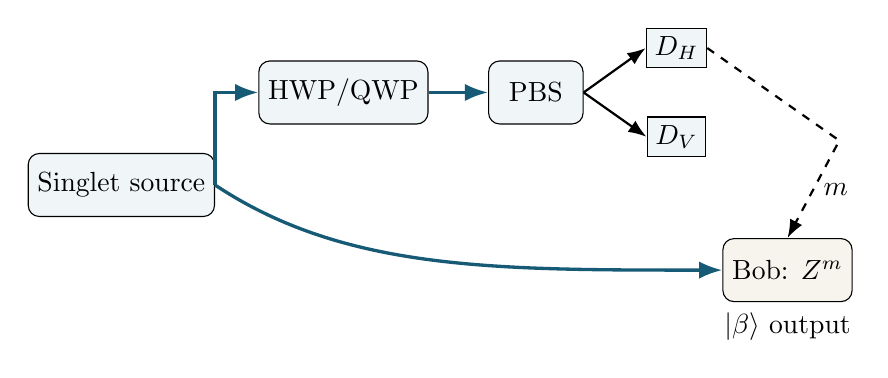
\begin{tikzpicture}[>=Latex,scale=0.94]
 \node[draw,rounded corners,fill=soft,minimum width=1.5cm,minimum height=.8cm] (src) at (0,0) {Singlet source};
 \node[draw,rounded corners,fill=soft,minimum width=1.55cm,minimum height=.8cm] (wp) at (3.0,1.25) {HWP/QWP};
 \node[draw,rounded corners,fill=soft,minimum width=1.2cm,minimum height=.8cm] (pbs) at (5.6,1.25) {PBS};
 \node[draw,rounded corners,fill=warm,minimum width=1.5cm,minimum height=.8cm] (corr) at (9.0,-1.15) {Bob: $Z^m$};
 \draw[very thick,accent,->] (src.east) |- (wp.west);
 \draw[very thick,accent,->] (wp.east)--(pbs.west);
 \draw[very thick,accent,->] (src.east) .. controls (3,-1.15) and (5,-1.15) .. (corr.west);
 \node[draw,fill=soft,inner sep=3pt] (d0) at (7.5,1.85) {$D_H$};
 \node[draw,fill=soft,inner sep=3pt] (d1) at (7.5,.65) {$D_V$};
 \draw[->,thick] (pbs.east) -- (d0.west);
 \draw[->,thick] (pbs.east) -- (d1.west);
 \draw[dashed,->,thick] (d0.east) -- (9.7,.6) -- (corr.north) node[midway,right] {$m$};
 \node[below] at (9,-1.6) {$\ket\beta$ output};
\end{tikzpicture}
\caption{One possible photonic remote state preparation apparatus. A classical detector message determines Bob's phase correction.}
\end{figure}

\subsubsection*{Part A3. General target on the Bloch sphere}
A general pure state is
\begin{equation}\ket{\beta'}=\cos\frac\theta2\ket H+\ee^{i\phi}\sin\frac\theta2\ket V.\end{equation}
Alice must now choose an \emph{arbitrary} polarisation measurement basis, not merely the equatorial rotation $R_{\hat n}(\pi/2)$. In optics, additional wave-plate control provides the independent polar angle $\theta$ as well as the azimuth $\phi$. With a singlet, projecting Alice onto the appropriate state remotely prepares $\ket{\beta'}$ at Bob for \emph{one} of her outcomes. The other outcome gives the orthogonal state $\ket{\beta'_{\perp}}$.

\textbf{Limitation worth explaining:} for arbitrary $\theta,\phi$, there is no single fixed correction such as $Z$ that maps $\ket{\beta'_{\perp}}$ into $\ket{\beta'}$ for \emph{every} target. The equatorial one-bit deterministic scheme relies on a special symmetry of that restricted ensemble. An experimental extension can therefore either (i) \emph{herald success} and accept one of the two outcomes, giving $1/2$ success with one bit, or (ii) use extra state-dependent feed-forward/classical communication or a general teleportation-style protocol to obtain deterministic arbitrary-state preparation. Changing wave plates alone is not sufficient to preserve the original deterministic one-bit guarantee for all Bloch-sphere states.

\subsubsection*{Part A4. Compare remote state preparation and teleportation}
Both protocols use pre-shared entanglement and classical communication; neither transmits an unknown qubit faster than light, and neither clones the original. The major distinctions are
\begin{center}\small
\begin{tabularx}{\linewidth}{@{}p{27mm}XX@{}}\toprule Feature&Equatorial remote state preparation&Standard qubit teleportation\\\midrule
Alice's knowledge&Alice knows $\phi$ and chooses her measurement&Alice need not know the input state\\
Quantum input&No unknown input qubit to transport&An actual unknown input qubit is consumed\\
Shared resource&One Bell pair&One Bell pair\\
Classical message&One bit for restricted equatorial ensemble&Two bits to specify four Bell-measurement outcomes\\
Bob's recovery&$I$ or $Z$ for this equatorial protocol&One of four Pauli corrections\\\bottomrule
\end{tabularx}\end{center}
Known-state preparation permits tailored measurement, which is why the restricted protocol can be cheaper in classical communication.

\subsubsection*{Part B. Continuous-variable (CV) teleportation: strengths and limitations}
CV teleportation encodes information in field quadratures $\hat x=(a+a^\dagger)/\sqrt2$ and $\hat p=(a-a^\dagger)/(i\sqrt2)$ rather than in a two-dimensional single-photon subspace. Alice and Bob share a \emph{two-mode squeezed entangled state}; Alice interferes the unknown optical mode with her half on a balanced beam splitter and makes two complementary homodyne measurements. She transmits continuous-valued classical measurement results, and Bob performs phase-space displacements to recover the state.

\textbf{Advantages.} Homodyne detectors can have high efficiency and are experimentally mature; the optical measurement and feed-forward can be nearly deterministic rather than relying on rare photon-counting events. The method works naturally with coherent/squeezed light and Gaussian optical states, and does not require resolving individual photons in each run.

\textbf{Limitations.} An ideal Einstein--Podolsky--Rosen resource would need infinite squeezing, which is unphysical. Finite squeezing adds noise to the teleported quadratures, decreasing fidelity. Optical loss, mode mismatch, detector inefficiency, imperfect squeezing and finite-bandwidth feed-forward also degrade the reconstructed state. CV Bell measurements still require classical communication (two real measurement outcomes), and deterministic \emph{Gaussian} processing alone does not provide universal fault-tolerant quantum computing.

For a standard unity-gain protocol teleporting unknown coherent states through a pure two-mode squeezed resource of squeezing $r$, a common idealised fidelity formula is
\begin{equation}\boxed{F_{\rm coh}=\frac{1}{1+\ee^{-2r}}.}\end{equation}
It gives the classical benchmark $F=1/2$ at $r=0$ and tends to 1 as squeezing grows, assuming the stated gain/noise conventions. This quantitative example illustrates the central trade-off: near-unit fidelity demands increasingly strong entanglement and increasingly low experimental noise.
\end{document}